\lab{Poisson's equation}{Poisson's equation}
\label{lab:poisson2d}

Suppose that we want to describe the distribution of heat throughout a region $\Omega$.
Let $h(x)$ represent the temperature on the boundary of $\Omega$ ($\partial \Omega$), and let $g(x)$ represent the initial heat distribution at time $t = 0$.
If we let $f(x,t)$ represent any heat sources/sinks in $\Omega$, then the flow of heat can be described by the boundary value problem (BVP)
\begin{align}
	\begin{split}
		& { } u_t = \triangle u + f(x,t), \quad x \in \Omega, \quad t >0,\\
		& { }u(x,t) = h(x), \quad x \in \partial \Omega, \\
		& { }u(x,0) = g(x).
	\end{split}
\end{align}
When the source term $f$ does not depend on time, there is often a steady-state heat distribution $u_{\infty}$ that is approached as $t \to \infty$.
This steady state $u_{\infty}$ is a solution of the BVP
\begin{align}
	\begin{split}
		& { }  \triangle u + f(x) = 0, \quad x \in \Omega,\\
		& { }u(x,t) = h(x), \quad x \in \partial \Omega.
	\end{split}
\end{align}

This last partial differential equation, $\triangle u = -f$, is called Poisson's equation.
This equation is satisfied by the steady-state solutions of many other evolutionary processes.
Poisson's equation is often used in electrostatics, image processing, surface reconstruction, computational fluid dynamics, and other areas.


\section*{Poisson's equation in two dimensions}

 Consider Poisson's equation together with Dirichlet boundary conditions on a square domain $R = [a,b]\times [c,d]$:
 \begin{align}
	\begin{split}
 	u_{xx} + u_{yy} &= f,\quad x \text{ in } R \subset \mathbb{R}^2,\\
 	u &= g, \quad x \text{ on } \partial R.
	\end{split}\label{eqn:2d_poisson}
\end{align}
Let $a = x_{-1}, x_0, \ldots, x_{N-1} = b$ be a partition of $[a,b]$, and let $c = y_{-1}, y_0, \ldots, y_{N-1} = d$ be a partition of $[c,d]$.
Suppose that there are $N+1$ evenly spaced points, so that $N$ is the number of subintervals in each dimension, and $x_i, y_j$ are given by
\begin{align*}
	x_i &= a + (i+1)h, \\
	y_j &= c + (j+1)h,
\end{align*}
for $i,j = 0, \ldots, N-2$, where $h = x_i-x_{i-1} = y_i-y_{i-1}$.
We look for an approximation $U_{i,\,j}$ on the grid $\{(x_i,y_j)\}_{i,j=-1}^{N-1}$.

Recall that
 \begin{align*}
 \triangle u &= u_{xx}(x,y) + u_{yy}(x,y) \\
&= \frac{u(x+h,y) - 2u(x,y)+ u(x-h,y)}{h^2} \\
 & \qquad{}+ 
 \frac{u(x,y+h) - 2u(x,y)+ u(x,y-h)}{h^2} + \mathcal{O}(h^2).
 \end{align*}
 We replace $\triangle $ with the finite difference operator $\triangle_h$, defined by
 \begin{align*}
 \triangle_h U_{ij} &= \frac{U_{i+1,\,j} - 2U_{i,\,j} + U_{i-1,\,j}}{h^2} + \frac{U_{i,\,j+1} - 2U_{i,\,j}+ U_{i,\,j-1}}{h^2},\\
&= \frac{1}{h^2}(U_{i-1,\,j} + U_{i+1,\,j} + U_{i,\,j-1} + U_{i,\,j+1}-4U_{i,\,j}).
 \end{align*}

 Then the set of equations  
\[
\triangle_h U_{ij} = f_{ij}, \quad i,j = 0,\ldots,N-2,
\]% $i,j = 1,\ldots,m$ 
can be written in matrix form as
 \[AU + p +  q  = f.\]

$A$ is a block tridiagonal matrix, given by 
\begin{align}
	\frac{1}{h^2}
\begin{bmatrix}
T & I & &  &\\
I &T & I & &\\
&\ddots  & \ddots & \ddots & \\
&  & I & T & I \\
&  &  & I & T\end{bmatrix}\label{poisson2d:matrixA}
\end{align}

where $I$ is the $N-1\times N-1$ % $m\times m$
identity matrix, and $T$ is the tridiagonal matrix
\[\begin{bmatrix}
-4 & 1 & &  &\\
1 &-4 & 1 & &\\
&\ddots  & \ddots & \ddots & \\
&  & 1 & -4 & 1 \\
&  &  & 1 & -4 \end{bmatrix}.\]


The vector $U$ is given by 
\[U = \begin{bmatrix} U^0 \\ U^1 \\ \\ U^{N-2} \end{bmatrix} \text{ where } U^j = 
\begin{bmatrix} U_{0,\,j} \\ U_{1,\,j} \\ \\ U_{N-2,\,j} \end{bmatrix} \text{ for each } j, \text{ }0\leq j \leq N-2.\]

% \[U = \begin{bmatrix} U^1 \\ U^2 \\ \\ U^m \end{bmatrix} \text{ where } U^j =
% \begin{bmatrix} U_{1,\,j} \\ U_{2,\,j} \\ \\ U_{m,\,j} \end{bmatrix} \text{ for each } j, 1\leq j \leq m\]
% So $U^j$ represents the $j$th row of interior points in our grid, where $y_j = jh$


The vectors $p$ and $q$ come from the boundary conditions of \eqref{eqn:2d_poisson}, and are given by 
\[p = \begin{bmatrix} p^0 \\ \ldots \\ \\ p^{N-2} \end{bmatrix}, \quad  q = \begin{bmatrix} q^0 \\ \ldots \\ \\ q^{N-2} \end{bmatrix},\]
where 
\[p^j = \frac{1}{h^2} \begin{bmatrix} g_{-1,\,j} \\ 0 \\ \vdots \\0\\ g_{N-1,\,j} \end{bmatrix} ,\,\,\, 0 \leq j \leq N-2,\]
and 
\[q^0 = \frac{1}{h^2}\begin{bmatrix} g_{0,-1}  \\ g_{1,-1} \\ \vdots \\ g_{N-3,-1}\\ g_{N-2,-1} \end{bmatrix}, \quad q^{N-2} = \frac{1}{h^2}\begin{bmatrix} g_{0,N-1} \\ g_{1,N-1} \\ \vdots \\ g_{N-3,N-1}\\ g_{N-2,N-1} \end{bmatrix}, \quad q^{j} = \begin{bmatrix} 0 \\ 0 \\ \vdots \\ 0 \\ 0 \end{bmatrix} ,\,\,\, 1 \leq j \leq N-3.\]

% The vector $q$ is given by $u = [q^0 \ldots q^{N-2}]^T$, %   $u = [q^1 \ldots q^m]^T$,
% where
% \[q^j = \frac{1}{h^2} \begin{bmatrix} g_{0,\,j} \\ 0 \\ \vdots \\0\\ g_{m+1,\,j} \end{bmatrix} , \,\,\, 2 \leq j \leq m-1\]
% and
% \[q^1 = \frac{1}{h^2}\begin{bmatrix} g_{1,0} + g_{0,1} \\ g_{2,0} \\ \vdots \\ g_{m-1,0}\\ g_{m,0} + g_{m+1,1}\end{bmatrix}, \quad q^m = \frac{1}{h^2}\begin{bmatrix} g_{1,m+1} + g_{0,m}\\ g_{2,m+1} \\ \vdots \\ g_{m-1,m+1}\\ g_{m,m+1} + g_{m+1,m}\end{bmatrix}\]




% \begin{problem}
% Find the solution $u$ of the 2D Poisson equation with the given Dirichlet boundary conditions:
% \begin{align*}
% 	\Delta u &= -\pi^2 \sin(\pi x)\sin(\pi y), \quad (x,y) \in [0,1]\times [0,1], \\
% 	u(x,0) &= 1-x, \\
% 	u(x,1) &= 1-2x, \\
% 	u(0,y) &= 1, \\
% 	u(1,y) &= -y.
% \end{align*}
%
% Graph your solution, and demonstrate convergence of the numerical approximation by
% creating a log-log plot of the error $E(h).$
% \end{problem}

% The matrix $A$ is sparse, and so we can use several functions from the package \texttt{scipy.sparse.linalg}.
% In particular, we use the functions \texttt{spdiags} and \texttt{spsolve}.
%
%  \begin{verbatim}
% D1,D2,D3 = -4*np.ones((1,m**2)), np.ones((1,m**2)), np.ones((1,m**2))
% Dm1, Dm2 = np.ones((1,m**2)), np.ones((1,m**2))
% for j in range(0,D2.shape[1]):
% 	if (j%m)==m-1:
% 		D2[0,j]=0
% 	if (j%m)==0:
% 		D3[0,j]=0
% diags = np.array([0,-1,1,-m,m])
% data = np.concatenate((D1,D2,D3,Dm1,Dm2),axis=0) # This stacks up rows
% A = 1./h**2.*spdiags(data, diags, m**2,m**2).asformat('csr') # This ap
%  \end{verbatim}

\begin{comment}
\subsection{2D Heat Equation}
Recall that the collection of finite difference equations
\[\nabla^2_h U_{ij} = 0, \quad 1 \leq i,j\leq m\]
can be written in matrix form as
\[AU + q  = 0\]

The Crank-Nicolson method for the 2D heat equation is given by
\[U_{i,\,j}^{n+1}- U_{i,\,j}^{n} = \frac{\Delta t}{2}(\nabla_h^2 U_{i,\,j}^{n} + \nabla_h^2 U_{i,\,j}^{n+1}) \text{ for each } 1 \leq i,j \leq m\]
is a second order accurate in both space and time. Basically we're using a midpoint scheme in time,
and a trapezoidal scheme in space. The resulting method is implicit, and can be written in matrix form as
\begin{align*}
	IU^{n+1} &= IU^n + \frac{\Delta t}{2}(AU^n + q + AU^{n+1} + q)\\
	(I - \frac{\Delta t}{2}A)U^{n+1}&= (I + \frac{\Delta t}{2}A)U^n + \Delta t q
\end{align*}

% TODO: What size must the time step be to ensure stability?

We will need to take many time steps, where many equations must be solved with the matrix $(I - \frac{\Delta t}{2}A)$.
The function \texttt{factorized} from \texttt{scipy.sparse.linalg} computes the LU decomposition of the matrix.
This decomposition reduces the time required for solving consecutive time steps.
\end{comment}

The following code implements the greater portion of the finite difference method; it leaves the construction of the matrix $A$ in \eqref{poisson2d:matrixA} to problem \ref{poisson2d:laplace}.

\begin{lstlisting}
from __future__ import division
from scipy.sparse import spdiags
from scipy.sparse.linalg import spsolve

def poisson_square(a1,b1,c1,d1,n,bcs, source): 
	# n = number of subintervals
	# We discretize in the x dimension by 
	# a1 = x_0 < x_1< ... < x_n=b1, and 
	# We discretize in the y dimension by 
	# c1 = y_0 < y_1< ... < y_n=d1. 
	# This means that we have interior points 
	# {x_1, ..., x_{n-1}}\times {y_1, ..., y_{n-1}}
	# or {x_1, ..., x_m}\times {y_1, ..., y_m} where m = n-1. 
	# In Python, this is indexed as 
	# {x_0, ..., x_{m-1}}\times {y_0, ..., y_{m-1}}
	# We will have m**2 pairs of interior points, and 
	# m**2 corresponding equations.
	# We will organize these equations by their 
	# y coordinates: all equations centered 
	# at (x_i, y_0) will be listed first, 
	# then (x_i, y_1), and so on till (x_i, y_{m-1})
	delta_x, delta_y, h, m = (b1-a1)/n, (d1-c1)/n, (b1-a1)/n, n-1
	
	####    Construct the matrix A    ####
	
	
	####    Here we construct the vector b    ####
	b, Array = np.zeros(m**2), np.linspace(0.,1.,m+2)[1:-1]
	# In the next line, source represents 
	# the inhomogenous part of Poisson's equation
	for j in xrange(m): 
		b[j*m:(j+1)*m] = source(a1+(b1-a1)*Array, c1+(j+1)*h*np.ones(m) )
	
    # In the next four lines, bcs represents the 
	# Dirichlet conditions on the boundary
	# y = c1+h, d1-h
	b[0:m] -= h**(-2.)*bcs(a1+(b1-a1)*Array,c1*np.ones(m))
	b[(m-1)*m:m**2] -= h**(-2.)*bcs(a1+(b1-a1)*Array,d1*np.ones(m))
	# x = a1+h, b1-h
	b[0::m] -= h**(-2.)*bcs(a1*np.ones(m),c1+(d1-c1)*Array) 
	b[(m-1)::m] -= h**(-2.)*bcs(b1*np.ones(m),c1+(d1-c1)*Array)
	
    ####    Here we solve the system A*soln = b    ####
	soln = spsolve(A,b) 
	
	# We return the solution, and the boundary values, 
	# in the array z.
	z = np.zeros((m+2,m+2) ) 
	for j in xrange(m): 
		z[1:-1,j+1] = soln[j*m:(j+1)*m]
	
	x, y = np.linspace(a1,b1,m+2), np.linspace(c1,d1,m+2)
	z[:,0], z[:,m+1]  = bcs(x,c1*np.ones(len(x)) ), bcs(x,d1*np.ones(len(x)) )
	z[0,:], z[m+1,:] = bcs(a1*np.ones(len(x)),y), bcs(b1*np.ones(len(x)),y)
	return z

\end{lstlisting}

\begin{problem}
Construct the matrix $A$ in \eqref{poisson2d:matrixA}. Make sure your matrix is sparse. Then use the code 
above to solve the boundary value problem
\begin{align}
	\begin{split}
	\Delta u = 0, &{}\quad x \in [0,1]\times [0,1],\\
	u(x,y) = x^3, &{}\quad (x,y) \in \partial ([0,1]\times [0,1]).
	\end{split}
	\label{poisson2d:laplace}
\end{align}
Plot the 3D solution with $n=100$.
\end{problem}

\begin{figure}
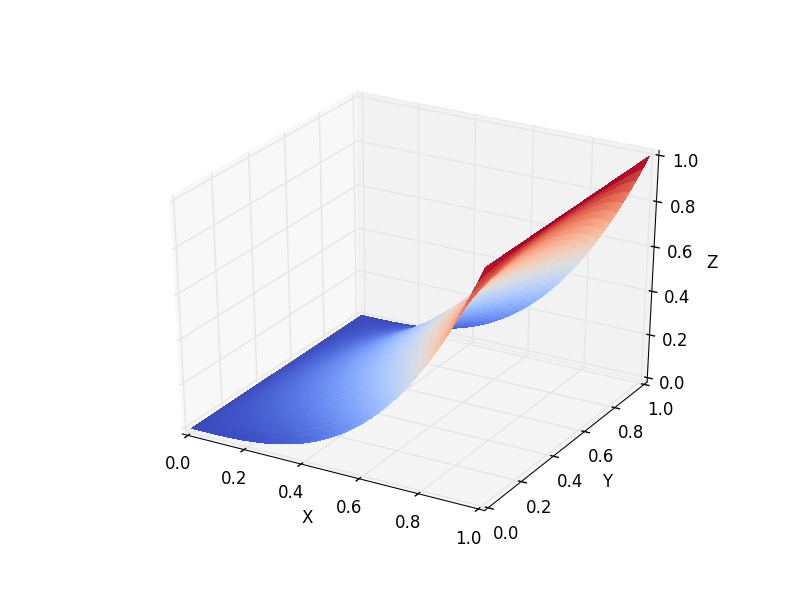
\includegraphics[width=\textwidth]{Laplace.png}
\caption{The solution of \eqref{poisson2d:laplace}.}
\end{figure}

\section*{Poisson's equation and conservative forces}
In physics Poisson's equation is used to describe the scalar potential of a conservative force.
In general
\[ \Delta V = - f\]
where $V$ is the scalar potential of the force, or the potential energy a particle would have at that point, and $f$ is a source term.
Examples of conservative forces include Newton's Law of Gravity (where matter become the source term) and Coulomb's Law, which gives the force between two charge particles (where charge is the source term).

In electrostatics the electric potential is also known as the voltage, and is denoted by $V.$ 
From Maxwell's equations it can be shown that that the voltage obeys Poisson's equation with the electric charge density (like a continuous cloud of electrons) being the source term: 
\[
 \Delta V = -\frac{\rho}{\epsilon_0},
\]
where $\rho$ is the charge density and $\epsilon_0$ is the permissivity of 
free space, which is a constant that we'll leave as $1$.

Usually a non zero $V$ at a point will cause a charged particle to move to a lower potential, changing $\rho$ and the solution to $V$.
However, in this analysis we'll assume that the charges are fixed in place.

Suppose we have 3 nested pipes.
The outer pipe is attached to "ground," which usually we define to be $V=0$, and the inner two have opposite relative charges.
Physically the two inner pipes would function like a capacitor.

The following code will plot the charge distribution of this setup.
\begin{lstlisting}
import matplotlib.colors as mcolors

def source(X,Y):
    """
    Takes arbitrary arrays of coordinates X and Y and returns an array of the same shape
    representing the charge density of nested charged squares
    """
    src = np.zeros(X.shape)
    src[ np.logical_or(
        np.logical_and( np.logical_or(abs(X-1.5) < .1,abs(X+1.5) < .1) ,abs(Y) < 1.6),
        np.logical_and( np.logical_or(abs(Y-1.5) < .1,abs(Y+1.5) < .1) ,abs(X) < 1.6))] = 1
    src[ np.logical_or(
        np.logical_and( np.logical_or(abs(X-0.9) < .1,abs(X+0.9) < .1) ,abs(Y) < 1.0),
        np.logical_and( np.logical_or(abs(Y-0.9) < .1,abs(Y+0.9) < .1) ,abs(X) < 1.0))] = -1
    return src

#Generate a color dictionary for use with LinearSegmentedColormap
#that places red and blue at the min and max values of data
#and white when data is zero

def genDict(data):
    zero = 1/(1 - np.max(data)/np.min(data))
    cdict = {'red':   [(0.0,  1.0, 1.0),
                   (zero,  1.0, 1.0),
                   (1.0,  0.0, 0.0)],
         'green': [(0.0,  0.0, 0.0),
                   (zero,  1.0, 1.0),
                   (1.0,  0.0, 0.0)],
         'blue':  [(0.0,  0.0, 0.0),
                   (zero,  1.0, 1.0),
                   (1.0,  1.0, 1.0)]}
    return cdict


a1 = -2.
b1 = 2.
c1 = -2.
d1 = 2.
n =100
X = np.linspace(a1,b1,n)
Y = np.linspace(c1,d1,n)
X,Y = np.meshgrid(X,Y)

plt.imshow(source(X,Y),cmap =  mcolors.LinearSegmentedColormap('cmap', genDict(source(X,Y))))
plt.colorbar(label="Relative Charge")
plt.show()
\end{lstlisting}

\begin{figure}
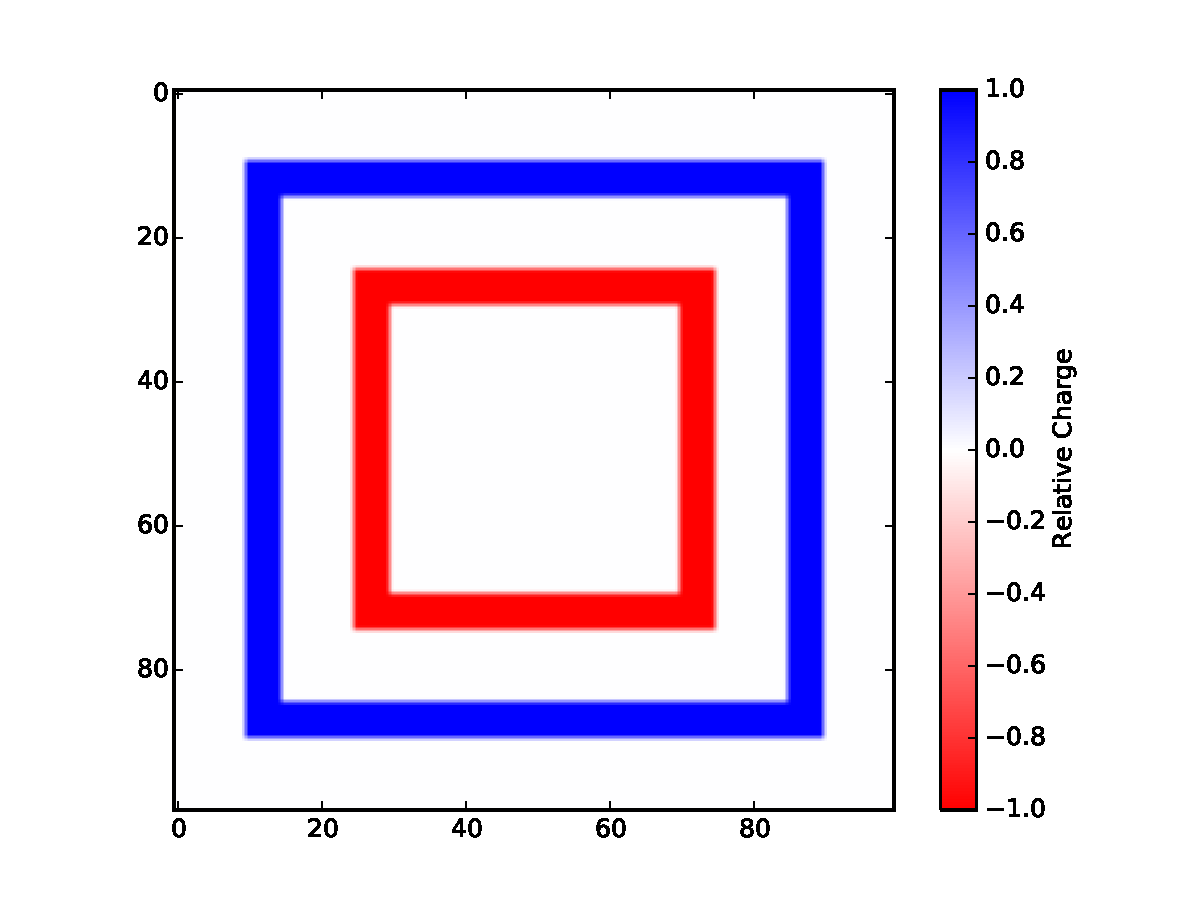
\includegraphics[width=\textwidth]{pipesRho.pdf}
\caption{The charge density of the 3 nested pipes.}
\end{figure}


The function \li{genDict} scales the color values to be white when the charge density is zero.
This is mostly to help visualize where there are neutrally charged zones by forcing them to be white.
You may find it useful to also apply it when you solve for the electric  potential.

With this definition of the charge density, we can solve Poisson's equation for the potential field.

\begin{problem}
Solve 
% \[\Delta V = -\rho(x,y)\]
\begin{align}
	\begin{split}
	\Delta V = -\rho(x,y), &{}\quad x \in [-2,2]\times [-2,2],\\
	u(x,y) = 0, &{}\quad (x,y) \in \partial ([-2,2]\times [-2,2]).
	\end{split}
	\label{poisson2d:source}
\end{align}
% 
for the electric potential $V.$
Use the source function ($-\rho$) defined above. % and grid sizes defined above.
% Use $V=0$ for the boundary conditions on all sides.
% \textit{(Due to the size of $A$, this is best done using sparse matrices)}
Plot the 2D solution using $n=100$.
\end{problem}

\begin{figure}
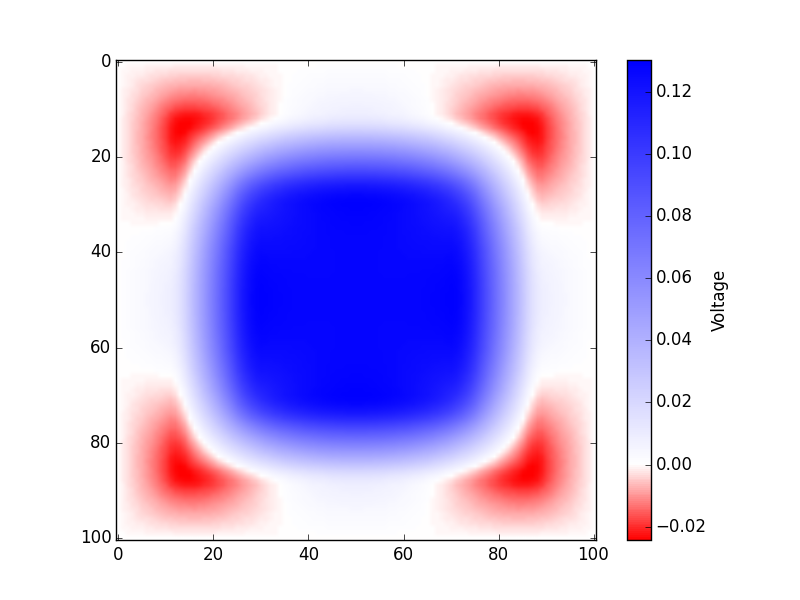
\includegraphics[width=\textwidth]{pipesV.png}
\caption{The electric potential of the 3 nested pipes.}
\end{figure}